\begin{statementbox}
\textbf{C090\quad 椭圆与双曲线共焦点的焦角--离心率关系}

设椭圆 $E$ 与双曲线 $H$ 均为非退化圆锥曲线，\textbf{有相同的两个焦点}
$F_1,F_2$，焦距 $F_1F_2=2c$（$c>0$），且 $P\in E\cap H$。
记
\[
\theta=\angle F_1PF_2\ (0<\theta<\pi),\qquad
0<e_1<1\quad(\text{椭圆}),\qquad e_2>1\quad(\text{双曲线}).
\]

\begin{center}
% 精确坐标：共焦点 F1=(-2,0), F2=(2,0)
% 椭圆 E: x^2/16 + y^2/12 = 1 (e1=1/2)
% 双曲线 H: x^2 - y^2/3 = 1 (e2=2)
% P=(2,3), PF1=5, PF2=3, F1F2=4, cos(theta)=3/5
% 所有几何点与图形由真实方程指定，并非自由手绘。
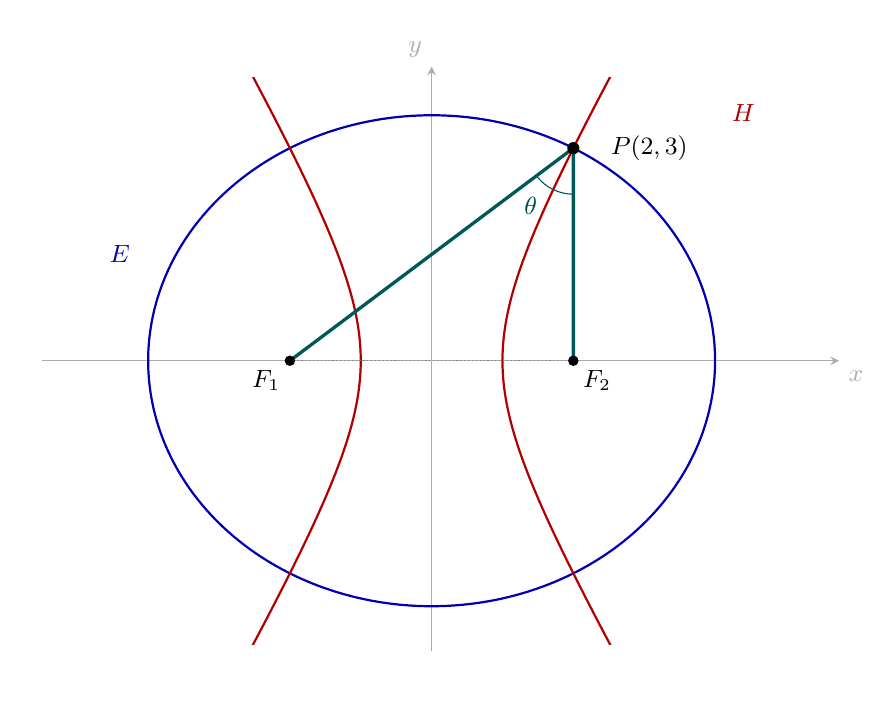
\begin{tikzpicture}[x=0.9cm,y=0.9cm,>=stealth,every node/.style={font=\small}]
  \path[use as bounding box] (-5.7,-4.5) rectangle (6.0,4.7);
  \draw[->,gray!65,thin] (-5.5,0)--(5.75,0) node[below right] {$x$};
  \draw[->,gray!65,thin] (0,-4.1)--(0,4.15) node[above left] {$y$};
  \begin{scope}
  \clip (-5.2,-4) rectangle (5.2,4);
  \draw[thick,blue!70!black,domain=0:360,samples=181,smooth,variable=\t]
    plot ({4*cos(\t)},{sqrt(12)*sin(\t)});
  \draw[thick,red!70!black,domain=-70:70,samples=131,smooth,variable=\t]
    plot ({1/cos(\t)},{sqrt(3)*tan(\t)});
  \draw[thick,red!70!black,domain=-70:70,samples=131,smooth,variable=\t]
    plot ({-1/cos(\t)},{sqrt(3)*tan(\t)});
  \end{scope}
  \coordinate (Fone) at (-2,0);
  \coordinate (Ftwo) at (2,0);
  \coordinate (PP) at (2,3);
  \draw[very thick,teal!70!black] (PP)--(Fone) (PP)--(Ftwo);
  \draw[thin,densely dotted,gray] (Fone)--(Ftwo);
  \fill[black] (Fone) circle(1.9pt) node[below left] {$F_1$};
  \fill[black] (Ftwo) circle(1.9pt) node[below right] {$F_2$};
  \fill[black] (PP) circle(2.2pt) node[right,xshift=10pt] {$P(2,3)$};
  \draw[teal!70!black] (2,2.35) arc[start angle=-90,end angle=-143.130102,radius=0.65];
  \node[teal!60!black] at (1.40,2.18) {$\theta$};
  \node[blue!70!black] at (-4.4,1.5) {$E$};
  \node[red!70!black] at (4.4,3.5) {$H$};
\end{tikzpicture}

\end{center}
\textbf{主结论：}
\[
\boxed{\frac{1-\cos\theta}{e_1^2}+
\frac{1+\cos\theta}{e_2^2}=2}
\quad\Longleftrightarrow\quad
\boxed{\frac{\sin^2(\theta/2)}{e_1^2}+
\frac{\cos^2(\theta/2)}{e_2^2}=1}.
\]
\medskip
\textbf{读懂主公式的入口：}同一个 $\triangle F_1PF_2$，椭圆固定
$PF_1+PF_2=2A$，双曲线固定 $|PF_1-PF_2|=2T$；
\emph{定和与定差确定两腰，焦角借余弦定理确定底边 $2c$}。
\end{statementbox}

\clearpage
\begin{statementbox}
\textbf{推论（焦角不等式）：}
\[
\boxed{\frac1{e_1}+\frac1{e_2}\le\frac2{\sin\theta}}
\quad\Longleftrightarrow\quad
\boxed{\sin\theta\le\frac{2e_1e_2}{e_1+e_2}}.
\]
\textbf{等号条件（必须同时满足）：}
\[
\boxed{e_1=\tan\frac\theta2,\qquad
 e_2=\cot\frac\theta2}\quad\Longleftrightarrow\quad
\boxed{e_1e_2=1\ \text{且}\ 0<\theta<\frac\pi2}.
\]
\textbf{注意：}在题设共焦且有公共点的前提下，$e_1e_2=1$
也等价于取到推论等号；此时 $\theta$ 必为锐角。
\textbf{几何等号：}若取焦点为 $(\pm c,0)$，等号时交点满足
$x=\pm c$，故焦点三角形在某个\emph{焦点}处为直角；
这与 $\angle F_1PF_2=\theta$ 为\emph{锐角}并不矛盾。
$\theta\ge\pi/2$ 时上述不等式严格。

\textbf{适用信号：}\emph{共焦点}、\emph{公共点}、\emph{焦点张角}、
\emph{椭圆和双曲线两种离心率}、\emph{证明含 $\sin\theta$ 的不等式}。

\medskip
\textbf{几何记号与范围（防止把两种 $a$ 混为一谈）。}
\[
 a_E=\frac{c}{e_1}>c,\qquad
 a_H=\frac{c}{e_2}<c,\qquad
 r_1=PF_1,\quad r_2=PF_2.
\]
椭圆焦半径\textbf{和固定}，双曲线焦半径\textbf{差的绝对值固定}：
\[
 \boxed{r_1+r_2=2a_E},\qquad
 \boxed{|r_1-r_2|=2a_H},\qquad F_1F_2=2c.
\]
这里 $a_E>a_H>0$，$P$ 不能落在两焦点连线上：
若在焦点外侧，$|r_1-r_2|=2c>2a_H$；
若在两焦点之间，$r_1+r_2=2c<2a_E$，均矛盾。
故 $0<\theta<\pi$，$\sin\theta>0$，推论中除以 $\sin\theta$ 合法。
\end{statementbox}
